%
% $Id: SANDExampleReportstrict.tex,v 1.28 2009-05-01 20:59:19 rolf Exp $
%
% This is an example LaTeX file which uses the SANDreport class file.
% It shows how a SAND report should be formatted, what sections and
% elements it should contain, and how to use the SANDreport class.
% It uses the LaTeX report class and the strict option.
%
% Get the latest version of the class file and more at
%    http://www.cs.sandia.gov/~rolf/SANDreport
%
% This file and the SANDreport.cls file are based on information
% contained in "Guide to Preparing {SAND} Reports", Sand98-0730, edited
% by Tamara K. Locke, and the newer "Guide to Preparing SAND Reports and
% Other Communication Products", SAND2002-2068P.
% Please send corrections and suggestions for improvements to
% Rolf Riesen, Org. 9223, MS 1110, rolf@cs.sandia.gov
%
% \documentclass[pdf,ps2pdf,12pt,report,strict,blank,OUO]{SANDreport}
\documentclass[pdf,ps2pdf,12pt,report,strict,blank,justified]{SANDreport}
\usepackage{pslatex}
\usepackage{mathptmx}	% Use the Postscript Times font
\usepackage[FIGBOTCAP,normal,bf,tight]{subfigure}
\usepackage{listings}
% \usepackage{enumitem}
% \usepackage{placeins}
\usepackage{caption}
% \usepackage{subcaption}
% \usepackage{draftwatermark}
% \SetWatermarkScale{.5}
% \SetWatermarkText{\shortstack{Draft \\[1em] Contains OUO}}
% \SetWatermarkText{\shortstack{Draft}}

% If you want to relax some of the SAND98-0730 requirements, use the "relax"
% option. It adds spaces and boldface in the table of contents, and does not
% force the page layout sizes.
% e.g. \documentclass[relax,12pt]{SANDreport}
%
% You can also use the "strict" option, which applies even more of the
% SAND98-0730 guidelines. It gets rid of section numbers which are often
% useful; e.g. \documentclass[strict]{SANDreport}
\usepackage{graphicx}
% \usepackage[table,xcdraw]{xcolor}

\pdfminorversion=7

\definecolor{dkgreen}{rgb}{0,0.6,0}
\definecolor{gray}{rgb}{0.5,0.5,0.5}
\definecolor{mauve}{rgb}{0.58,0,0.82}


% ---------------------------------------------------------------------------- %
%
% Set the title, author, and date
%
    \title{Balar: A SST GPU Component for \\Performance Modeling and Profiling}

    \author{C. Hughes$^2$, S. Hammond$^2$, M. Zhang$^1$ \\
            M. Khairy$^1$, T. Rogers$^1$, and R.J. Hoekstra$^2$ \\
            \small{$^1$AALP Research Group, Purdue University, West Lafayette, IN 47907} \\
            \small{$^2$Center for Computing Research, Sandia National Laboratories, Albuquerque, NM 87185} \\
           }

    % There is a "Printed" date on the title page of a SAND report, so
    % the generic \date should generally be empty.
    \date{}


% ---------------------------------------------------------------------------- %
% Set some things we need for SAND reports. These are mandatory
%
\SANDnum{SAND2019-10389}
\SANDprintDate{\today}
\SANDauthor{C. Hughes, S.D. Hammond, and R.J. Hoekstra \\
            Center for Computing Research \\
            Sandia National Laboratories \\
            Albuquerque, NM 87185 \\
            \{chughes, sdhammo, rjhoeks\}@sandia.gov \\
            \\
            M. Zhang, M. Khairy, and T. Rogers \\
            Accelerator Architecture Lab \\
            Purdue University \\
            West Lafayette, IN 47907 \\
            {zhan2308@purdue.edu, khairy2011@gmail.com, timrogers@purdue.edu}
            }

% ---------------------------------------------------------------------------- %
% The Style Guide doesn't require it, but if you really want to mark your cover
% page as UUR, uncomment this
\SANDmarkReleaseUUR


% ---------------------------------------------------------------------------- %
% The following definition does not have a default value and will not
% print anything, if not defined
%
% \SANDsupersed{SAND1901-0001}{January 1901}
% \input{MarkOUO}


% ---------------------------------------------------------------------------- %
% Adjust floats
%
\setlength{\textfloatsep}{+18pt}
\setlength\abovecaptionskip{-6pt}

% ---------------------------------------------------------------------------- %
%
% Start the document
%
\begin{document}
    \maketitle

    % ------------------------------------------------------------------------ %
    % An Abstract is required for SAND reports
    %
    \begin{abstract}
       Programmable accelerators have become commonplace in modern computing systems.
Advances in programming models and the availability of unprecedented amounts of data
have created a space for massively parallel accelerators capable of maintaining
context for thousands of concurrent threads resident on-chip. These threads are
grouped and interleaved on a cycle-by-cycle basis among several massively
parallel computing cores. One path for the design of future supercomputers
relies on an ability to model the performance of these massively parallel cores
at scale.

The SST framework has been proven to scale up to run simulations containing tens
of thousands of nodes. A previous report described the initial integration of
the open-source, execution-driven GPU simulator, GPGPU-Sim, into the SST
framework. This report discusses the results of the integration and how to use
the new GPU component in SST. It also provides examples of what it can be used
to analyze and a correlation study showing how closely the execution matches
that of a Nvidia V100 GPU when running kernels and mini-apps.

    \end{abstract}

    % ------------------------------------------------------------------------ %
    % An Acknowledgement section is optional but important, if someone made
    % contributions or helped beyond the normal part of a work assignment.
    % Use \section* since we don't want it in the table of context
    %
    \clearpage
    \section*{Acknowledgment}
      \input{sst_gpgpu_perf_ack}


    % ------------------------------------------------------------------------ %
    % The table of contents and list of figures and tables
    % Comment out \listoffigures and \listoftables if there are no
    % figures or tables. Make sure this starts on an odd numbered page
    %
    \cleardoublepage          % TOC needs to start on an odd page
    \tableofcontents
    \listoffigures
    \listoftables

    % ---------------------------------------------------------------------- %
    % An optional preface or Foreword
%     \clearpage
%     \section*{Preface}
%     \addcontentsline{toc}{section}{Preface}
%       \input{CommonPreface}


    % ---------------------------------------------------------------------- %
    % An optional executive summary
%     \clearpage
%     \section*{Summary}
%     \addcontentsline{toc}{section}{Summary}
%       \input{CommonSummary}


    % ---------------------------------------------------------------------- %
    % An optional glossary. We don't want it to be numbered
%     \clearpage
%     \section*{Nomenclature}
%     \addcontentsline{toc}{section}{Nomenclature}
%     \begin{description}
%       \item[dry spell]
%           using a dry erase marker to spell words
%       \item[dry wall]
%           the writing on the wall
%       \item[dry humor]
%           when people just do not understand
%
%           \item[DRY]
%           Don't Repeat Yourself
%     \end{description}


    % ---------------------------------------------------------------------- %
    % This is where the body of the report begins; usually with an Introduction
    %
    \SANDmain           % Start the main part of the report

   \chapter{Introduction}
      \label{ch:intro}
      As the architectures of high-performance computing (HPC) evolves, there is a growing
need to understand and quantify the performance and design benefits of
emerging technologies. To complicate the design space, the rise of
General-Purpose Graphics Processing Units (GPGPUs) and other compute
accelerators, which are needed to handle the growing demands of compute-heavy
workloads, have become a necessary component in both high-performance
supercomputers and datacenter-scale systems. That the first exascale machines
will leverage the massively parallel compute capabilities of GPUs
\cite{snl_roadmap, ornl_roadmap, llnl_roadmap} is indicative of the growing
necessity of accelerator-based node architectures to obtain high compute
throughputs. As the software stack and
programming model of GPUs and their peer accelerators continue to improve, there
is every indication that this trend of accelerator integration will continue,
leading to a diverse ecosystem of technologies. GPUs are likely to continue to
play a role as discrete accelerators or integrated as a part of an SOC. As a
result, architects who wish to study the design of large-scale systems will need
to evaluate system and software designs using a GPU model. However, the focus of
all publicly available cycle-level simulators ({\em e.g.} GPGPU-Sim~\cite{gpgpu_sim})
to date has been on single-node performance. In order to truly study the problem at scale,
and to permit larger workloads to be evaluated, a parallelizable, multi-node GPU
simulator is necessary.

The Structural Simulation Toolkit (SST)~\cite{sst} is a parallel discrete
event-driven simulation framework that provides an infrastructure capable of
modeling a variety of high performance computing systems at many different
scales. Currently used by a wide variety of government agencies and computer
manufacturers to design and simulate HPC architectures, and, supported by a
Python and C++ code base with a large array of customization options, SST offers
the HPC community powerful, highly customizable, tools to create and integrate
models for evaluating current and future HPC node architectures and interconnect
networks. What has been lacking, up to this point, has been a method
to integrate accelerators into a node model in SST. This report builds upon
previous work~\cite{sst_gpgpu}, providing more details on our efforts to
integrate an open-source GPGPU simulator, GPGPU-Sim, into SST. This integration effort
will provide SST users the ability to run GPGPU-based simulations using the Balar
GPU component and will serve as a model for future accelerator integration
studies.



   \chapter{GPGPU-Sim Integration With SST}
      \label{ch:integration}
      The latest version of GPGPU-Sim is a (mostly) object-oriented design written in
C++ with a sharp delineation between the functional and timing models of the
system.
A high-level overview of the organization is shown in Figure
\ref{fig:gpgpusim_top}. The SIMT blocks can be thought of as NVIDIA-like Streaming
Multiprocessors (SMs) or AMD-like Compute Units (CUs). The interconnect is currently
a modified
version of BookSim~\cite{booksim}, which can model a variety of topologies, and
the memory partition is a custom model. The remainder of this section describes
the integration of GPGPU-Sim with SST.

   \begin{figure}[!htb]
      \centering
      \setlength{\abovecaptionskip}{6pt plus 1pt minus 1pt}
      \includegraphics[width=.85\textwidth,keepaspectratio]{figures/gpgpusim_top.png}
      \captionsetup{format=hang, justification=centering, width=.75\textwidth}
      \caption[Overall GPGPU-Sim Architecture]{Overall GPGPU-Sim Architecture \protect\cite{gpgpu_sim}}
      \label{fig:gpgpusim_top}
   \end{figure}

\section{Scheduler}
\label{sec:sched}
The first step in integrating GPGPU-Sim into SST is to handle the interaction
with a SST CPU component. Since GPUs today function solely as co-processors,
functionally executing GPU-enabled binaries requires the CPU to initialize and
launch kernels of work to the GPU. In our model, the GPU is constructed out of
two discrete SST components -- a scheduler and a SM block~\cite{v100}. A block
diagram of the model is shown in Figure~\ref{fig:gpu_sched}. When CUDA functions
are called from the CPU component, they are intercepted and translated into
messages that are transfered by SST links to the GPU (along with the associated
parameters).

The CPU component (Ariel in the initial implementation) is connected via SST
links to 2 GPU components: the SMs, which implement the timing and functional
model for the GPU cores, and a centralized kernel and CTA scheduler (GPUSched).
When CUDA calls are intercepted from the CPU, messages are sent to both the SMs
and the GPU scheduler. Messages related to memory copies and other information
necessary to populate the GPU functional model are sent directly to the SM
elements, since the functional model for executing the GPU kernels lives inside
the SM elements. Calls related to enqueuing kernels for execution are sent to
the GPU scheduler element, which co-ordinates the launching of CTAs on the SMs,
{\em e.g.} \texttt{cudaConfigureCall} and \texttt{cudaLaunch}.


   \begin{figure}[!htb]
      \centering
      \setlength{\abovecaptionskip}{6pt plus 1pt minus 1pt}
      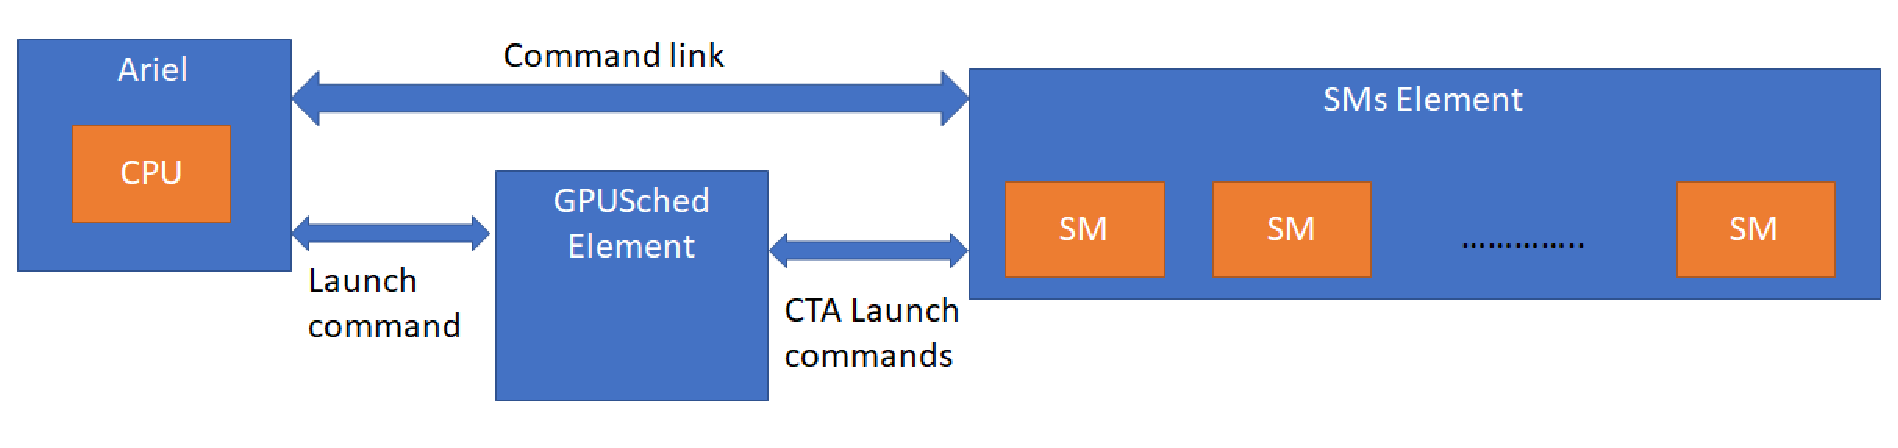
\includegraphics[width=.95\textwidth,keepaspectratio]{figures/sched.eps}
      \captionsetup{format=hang, justification=centering, width=1.0\textwidth}
      \caption{SST Element Architecture for Kernel/CTA Scheduler and SMs Components}
      \label{fig:gpu_sched}
   \end{figure}


As CTAs complete on the SMs, messages are sent back to the GPU scheduler
element, which pushes new work to the SMs from enqueued kernels as needed.
Memory copies from the CPU to GPU address space are handled on a configurable
page-size granularity, similar to how conventional CUDA unified memory handles
the transfer of data from CPU to GPU memories.


   \begin{figure}[!htb]
      \centering
      \setlength{\abovecaptionskip}{6pt plus 1pt minus 1pt}
      \includegraphics[width=.75\textwidth,keepaspectratio]{figures/scheduler.eps}
      \captionsetup{format=hang, justification=centering, width=.75\textwidth}
      \caption{Centralized GPU Scheduler Component}
      \label{fig:sched}
   \end{figure}


The centralized GPU scheduler receives kernel launch commands from the CPU, then
issues CTA launch commands to the SMs. The scheduler also receives notifications
from the SMs when the CTAs finish. The reception of kernel launch and CTA
complete notifications are independent, therefore we designed a different
handler for each type of message. Figure~\ref{fig:sched} shows the design of the
centralized kernel and CTA Scheduler. The kernel handler listens to calls from a
CPU component and pushes kernel launch information to the kernel queue when it
receives kernel configure and launch commands. The SM map table contains CTA
slots for each of the SMs, which is reserved when launching a CTA and released when a
message indicating that a CTA has finished is received from the SMs. The
scheduler clock ticks trigger CTA launches to SMs, when space is available and
there is a pending kernel. On every tick, the scheduler issues a CTA launch
command for currently unfinished kernels if any CTA slot is available or tries
to fetch a new kernel launch from kernel queue. The CTA handler also waits for
SMs to reply the CTA finish message, so that CTA slots in the SM map table may
be freed.


\section{Streaming-Multiprocessor}
\label{sec:sms}
To support the GPGPU-Sim functional model, a number of the simulator's overloaded
CUDA Runtime API calls were updated. A number of functions that originally assumed
the application and simulator were within same address space now support them being
decoupled. Initialization functions, such as \texttt{\textunderscore \textunderscore
cudaRegisterFatBinary}, now take paths to the original application to obtain the PTX
assembly of CUDA kernels.

   \begin{figure}[!htb]
      \centering
      \setlength{\abovecaptionskip}{6pt plus 1pt minus 1pt}
      \includegraphics[width=.90\textwidth,keepaspectratio]{figures/transfer_flow.png}
      \captionsetup{format=hang, justification=centering, width=.75\textwidth}
      \caption{SST Link and IPCTunnels for Functional Model Support}
      \label{fig:gpu_transfer_model}
   \end{figure}


Supporting the functional model of GPGPU-Sim also requires transferring values
from the executing CPU application to the GPU memory system. This is solved by leveraging
the inter-process communication tunnel framework from SST-Core, as shown in
Figure~\ref{fig:gpu_transfer_model}. Chunks of memory are transferred from the CPU
application to the GPU memory system at the granularity of a standard memory page (4KiB). The
transfer of pages is a blocking operation, therefore all stores to the GPU
memory system must be completed before another page is transferred or another
API call is processed.

To complete the integration with SST, everything except the SIMT units are
replaced with SST components, as shown in Figure~\ref{fig:gpgpu_sst}. The host
CPU is swapped for a SST execution component, such as Ariel or Juno. The
interconnect is swapped for a SST networking component, such as Shogun,
Kingsley, or Merlin. The memory partition, caches, and ports are swapped for
SST memHierarchy components -- caches and backing store models such as
TimingDRAM, SimpleMem, or CramSim. A detailed description of how to use the GPU
component can be found in~\cite{sst_gpgpu}. The remainder of this paper is
dedicated to a discussion of performance.


   \begin{figure}[!htb]
      \centering
      \setlength{\abovecaptionskip}{6pt plus 1pt minus 1pt}
      \includegraphics[width=.85\textwidth,keepaspectratio]{figures/sst_gpgpusim_top.png}
      \captionsetup{format=hang, justification=centering, width=.75\textwidth}
      \caption{SST GPGPU-Sim Integration}
      \label{fig:gpgpu_sst}
   \end{figure}



   \chapter{Performance Analysis}
      \label{sec:performance}
      This chapter is devoted to an analysis of the functional and timing models in
SST when using the GPU component as a part of a generalized compute node. Since
GPUs in HPC function solely as co-processors, functionally executing GPU-enabled
binaries requires the CPU to initialize and launch kernels of work to the GPU.
Figure~\ref{fig:sst_volta} shows the general simulation model used for the evaluation.
The Command Link and Data Link serve as the transport mechanism for the CPU (host)
to launch and coordinate work with the GPU (device). The other components in each
model can be tailored to fit any host and device that one wishes to model.

   \begin{figure}[!htb]
      \centering
      \setlength{\abovecaptionskip}{6pt plus 1pt minus 1pt}
      \includegraphics[width=.95\textwidth,keepaspectratio]{figures/sst_v100_model.png}
      \captionsetup{format=hang, justification=centering, width=.75\textwidth}
      \caption{SST Model of CPU With GPU Attached}
      \label{fig:sst_volta}
   \end{figure}

\section{Functional Testing}
The functional correctness of the model was validated using the unit tests from
the Kokkos Kernels suite~\cite{kokkos_kernels}. The unit tests were compiled
using the parameters in Table~\ref{tab:kokkos_build}. The target node
architecture was assumed to be an Intel Broadwell attached to an NVIDIA Pascal
GPUs. This target architecture was chosen based on hardware availability,
specifically Sandia's Doom cluster, which is based on the CTS-1
procurement. The SST model is derived from Figure~\ref{fig:sst_volta} using the
model parameters in Table`\ref{tab:p100_params} to represent an NVIDIA P100
SXM2~\cite{p100}.

    \begin{table}[!htbp]
        \centering
        \setlength{\abovecaptionskip}{6pt plus 1pt minus 1pt}
        \captionsetup{width=.75\textwidth}
        \caption{Kokkos Build Parameters}
        \begin{tabular}{|l|}
            \hline
            KOKKOSKERNELS\_SCALARS=double          \\ \hline
            KOKKOSKERNELS\_LAYOUTS=left            \\ \hline
            KOKKOSKERNELS\_ORDINALS=int            \\ \hline
            KOKKOSKERNELS\_OFFSETS=int             \\ \hline
            KOKKOSKERNELS\_DEVICES=Cuda     	   \\ \hline
            KOKKOS\_ARCH=Pascal60              	   \\ \hline
         \end{tabular}
        \label{tab:kokkos_build}
    \end{table}

    \begin{table}[!htbp]
      \centering
      \setlength{\abovecaptionskip}{6pt plus 1pt minus 1pt}
      \captionsetup{width=.75\textwidth}
      \caption{Broadwell/P100 Model Parameters}
      \subtable[CPU]{%
         \begin{tabular}{|l|c|}
            \hline
            Clock                   & 1200MHz  \\ \hline
            DDR Clock               & 2400     \\ \hline
            DDR Capactiy            & 16384MiB \\ \hline
            Mesh Frequency          & 800MHz   \\ \hline
            Mesh Input Ports        & 1        \\ \hline
            Mesh Output Ports       & 1        \\ \hline
            Data Link Latency       & 23840ps  \\ \hline
            Command Link Latency    & 23840ps  \\ \hline
         \end{tabular}
      }
      \hspace{1cm}
      \subtable[GPU]{%
         \begin{tabular}{|l|c|}
            \hline
            Clock                 & 1328MHz          \\ \hline
            SMs                   & 56               \\ \hline
            L2 Slices             & 8                \\ \hline
            L2 Capactiy           & 512KiB per slice \\ \hline
            HBM Capacity          & 16384MiB         \\ \hline
            HBM Stacks            & 4                \\ \hline
            Crossbar Frequency    & 1000MHz          \\ \hline
            Crossbar Input Ports  & 2                \\ \hline
            Crossbar Output Ports & 1                \\ \hline
         \end{tabular}
      }
      \label{tab:p100_params}
   \end{table}

Table~\ref{tab:kokkos_tests} shows the Kokkos Kernels unit tests that were run.
With the current implementation of SST-GPU, 46 out of 94 tests run to completion
and pass. The passing tests are highlighted in green. Of the remaining tests,
red tests fail in both SST-GPGPU and GPGPU-Sim due to the wrong value from gpu simulation. The tests in pink
failed previously because the PTX parser cannot locate a post-dominator. Now since
the the target configuration for Kokkos compilation has been changed 
to aiming at only GPUs, these tests no longer exist. There
are plans to work with the Kokkos Kernels developers to find a solution. The
tests in yellow sometimes fail because of a bug in the SST that randomly causes double free. 
The SST developers should be able to locate the problem. The tests in blue did not exist previously but now fail 
because the current SST does not support cudaCreateTextureObject function. 
The three remaining tests, in purple, run to completion
and pass in GPGPU-Sim but have run for more than 7 days without completion in SST. It is believed that they would complete successfully if given more run time.

   \begin{table}[!htbp]
      \centering
      \setlength{\belowcaptionskip}{6pt plus 1pt minus 1pt}
      \captionsetup{width=.75\textwidth}
      \caption{Kokkos Kernels Unit Test Results}
      \resizebox{\columnwidth}{!}{
         \begin{tabular}{|>{\columncolor[HTML]{34FF34}}l |l|}
            \hline
            1                          & abs\_double                                                         \\ \hline
            2                          & abs\_mv\_double                                                     \\ \hline
            3                          & asum\_double                                                        \\ \hline
            4                          & axpby\_double                                                       \\ \hline
            5                          & axpby\_mv\_double                                                   \\ \hline
            6                          & axpy\_double                                                        \\ \hline
            7                          & axpy\_mv\_double                                                    \\ \hline
            8                          & dot\_double                                                         \\ \hline
            9                          & dot\_mv\_double                                                     \\ \hline
            10                         & mult\_double                                                        \\ \hline
            11                         & mult\_mv\_double                                                    \\ \hline
            12                         & nrm1\_double                                                        \\ \hline
            13                         & nrm1\_mv\_double                                                    \\ \hline
            14                         & nrm2\_double                                                        \\ \hline
            15                         & nrm2\_mv\_double                                                    \\ \hline
            16                         & nrm2\_squared\_double                                               \\ \hline
            17                         & nrm2\_squared\_mv\_double                                           \\ \hline
            \cellcolor[HTML]{FE0000}18 & nrminf\_double                                                      \\ \hline
            \cellcolor[HTML]{FE0000}19 & nrminf\_mv\_double                                                  \\ \hline
            \cellcolor[HTML]{FE0000}20 & reciprocal\_double                                                  \\ \hline
            \cellcolor[HTML]{FE0000}21 & reciprocal\_mv\_double                                              \\ \hline
            22                         & scal\_double                                                        \\ \hline
            23                         & scal\_mv\_double                                                    \\ \hline
            24                         & sum\_double                                                         \\ \hline
            25                         & sum\_mv\_double                                                     \\ \hline
            26                         & update\_double                                                      \\ \hline
            27                         & update\_mv\_double                                                  \\ \hline
            \cellcolor[HTML]{D1B3FF}28 & gemv\_double                                                        \\ \hline
            \cellcolor[HTML]{D1B3FF}29 & gemm\_double                                                        \\ \hline
            \cellcolor[HTML]{FF00FF}30 & sparse\_spgemm\_double\_int\_int\_TestExecSpace                     \\ \hline
            \cellcolor[HTML]{FF00FF}31 & sparse\_spadd\_double\_int\_int\_TestExecSpace                      \\ \hline
            \cellcolor[HTML]{FF00FF}32 & sparse\_gauss\_seidel\_double\_int\_int\_TestExecSpace              \\ \hline
            \cellcolor[HTML]{FF00FF}33 & sparse\_block\_gauss\_seidel\_double\_int\_int\_TestExecSpace       \\ \hline
            \cellcolor[HTML]{FF00FF}34 & sparse\_crsmatrix\_double\_int\_int\_TestExecSpace                  \\ \hline
            \cellcolor[HTML]{FF00FF}35 & sparse\_blkcrsmatrix\_double\_int\_int\_TestExecSpace               \\ \hline
            \cellcolor[HTML]{FF00FF}36 & sparse\_replaceSumIntoLonger\_double\_int\_int\_TestExecSpace       \\ \hline
            \cellcolor[HTML]{FF00FF}37 & sparse\_replaceSumInto\_double\_int\_int\_TestExecSpace             \\ \hline
            \cellcolor[HTML]{FF00FF}38 & graph\_graph\_color\_double\_int\_int\_TestExecSpace                \\ \hline
            \cellcolor[HTML]{FF00FF}39 & graph\_graph\_color\_deterministic\_double\_int\_int\_TestExecSpace \\ \hline
            \cellcolor[HTML]{FF00FF}40 & graph\_graph\_color\_d2\_double\_int\_int\_TestExecSpace            \\ \hline
            \cellcolor[HTML]{FF00FF}41 & common\_ArithTraits                                                 \\ \hline
            42                         & common\_set\_bit\_count                                             \\ \hline
            43                         & common\_ffs                                                         \\ \hline
            \cellcolor[HTML]{FE0000}44 & batched\_scalar\_serial\_set\_double\_double                        \\ \hline
            45                         & batched\_scalar\_serial\_scale\_double\_double                      \\ \hline
            46                         & batched\_scalar\_serial\_gemm\_nt\_nt\_double\_double               \\ \hline
            47                         & batched\_scalar\_serial\_gemm\_t\_nt\_double\_double                \\ \hline
            \end{tabular}

            \hspace{1cm}

            \begin{tabular}{|>{\columncolor[HTML]{34FF34}}l |l|}
            \hline
            48                         & batched\_scalar\_serial\_gemm\_nt\_t\_double\_double                \\ \hline
            49                         & batched\_scalar\_serial\_gemm\_t\_t\_double\_double                 \\ \hline
            50                         & batched\_scalar\_serial\_trsm\_l\_l\_nt\_u\_double\_double          \\ \hline
            \cellcolor[HTML]{FE0000}51 & batched\_scalar\_serial\_trsm\_l\_l\_nt\_n\_double\_double          \\ \hline
            52                         & batched\_scalar\_serial\_trsm\_l\_u\_nt\_u\_double\_double          \\ \hline
            \cellcolor[HTML]{FE0000}53 & batched\_scalar\_serial\_trsm\_l\_u\_nt\_n\_double\_double          \\ \hline
            54                         & batched\_scalar\_serial\_trsm\_r\_u\_nt\_u\_double\_double          \\ \hline
            \cellcolor[HTML]{FE0000}55 & batched\_scalar\_serial\_trsm\_r\_u\_nt\_n\_double\_double          \\ \hline
            \cellcolor[HTML]{FF00FF}56 & batched\_scalar\_serial\_trsm\_l\_l\_t\_u\_double\_double           \\ \hline
            \cellcolor[HTML]{FF00FF}57 & batched\_scalar\_serial\_trsm\_l\_l\_t\_n\_double\_double           \\ \hline
            \cellcolor[HTML]{FF00FF}58 & batched\_scalar\_serial\_trsm\_l\_u\_t\_u\_double\_double           \\ \hline
            \cellcolor[HTML]{FF00FF}59 & batched\_scalar\_serial\_trsm\_l\_u\_t\_n\_double\_double           \\ \hline
            60                         & batched\_scalar\_serial\_gemv\_nt\_double\_double                   \\ \hline
            61                         & batched\_scalar\_serial\_gemv\_t\_double\_double                    \\ \hline
            62                         & batched\_scalar\_serial\_trsv\_l\_nt\_u\_double\_double             \\ \hline
            \cellcolor[HTML]{FE0000}63 & batched\_scalar\_serial\_trsv\_l\_nt\_n\_double\_double             \\ \hline
            64                         & batched\_scalar\_serial\_trsv\_u\_nt\_u\_double\_double             \\ \hline
            \cellcolor[HTML]{FE0000}65 & batched\_scalar\_serial\_trsv\_u\_nt\_n\_double\_double             \\ \hline
            \cellcolor[HTML]{FE0000}66 & batched\_scalar\_team\_set\_double\_double                          \\ \hline
            67                         & batched\_scalar\_team\_scale\_double\_double                        \\ \hline
            \cellcolor[HTML]{F8FF00}68 & batched\_scalar\_team\_gemm\_nt\_nt\_double\_double                 \\ \hline
            \cellcolor[HTML]{F8FF00}69 & batched\_scalar\_team\_gemm\_t\_nt\_double\_double                  \\ \hline
            \cellcolor[HTML]{F8FF00}70 & batched\_scalar\_team\_gemm\_nt\_t\_double\_double                  \\ \hline
            71                         & batched\_scalar\_team\_gemm\_t\_t\_double\_double                   \\ \hline
            72                         & batched\_scalar\_team\_trsm\_l\_l\_nt\_u\_double\_double            \\ \hline
            73                         & batched\_scalar\_team\_trsm\_l\_l\_nt\_n\_double\_double            \\ \hline
            74                         & batched\_scalar\_team\_trsm\_l\_u\_nt\_u\_double\_double            \\ \hline
            \cellcolor[HTML]{FE0000}75 & batched\_scalar\_team\_trsm\_l\_u\_nt\_n\_double\_double            \\ \hline
            76                         & batched\_scalar\_team\_trsm\_r\_u\_nt\_u\_double\_double            \\ \hline
            \cellcolor[HTML]{FE0000}77 & batched\_scalar\_team\_trsm\_r\_u\_nt\_n\_double\_double            \\ \hline
            \cellcolor[HTML]{FF00FF}78 & batched\_scalar\_team\_trsm\_l\_l\_t\_u\_double\_double             \\ \hline
            \cellcolor[HTML]{FF00FF}79 & batched\_scalar\_team\_trsm\_l\_l\_t\_n\_double\_double             \\ \hline
            \cellcolor[HTML]{FF00FF}80 & batched\_scalar\_team\_trsm\_l\_u\_t\_u\_double\_double             \\ \hline
            \cellcolor[HTML]{FF00FF}81 & batched\_scalar\_team\_trsm\_l\_u\_t\_n\_double\_double             \\ \hline
            82                         & batched\_scalar\_team\_gemv\_nt\_double\_double                     \\ \hline
            83                         & batched\_scalar\_team\_gemv\_t\_double\_double                      \\ \hline
            \cellcolor[HTML]{F8FF00}84 & batched\_scalar\_serial\_lu\_double                                 \\ \hline
            \cellcolor[HTML]{FF00FF}85 & batched\_scalar\_serial\_inverselu\_double                          \\ \hline
            \cellcolor[HTML]{FF00FF}86 & batched\_scalar\_serial\_solvelu\_double                            \\ \hline
            \cellcolor[HTML]{D1B3FF}87 & batched\_scalar\_team\_lu\_double                                   \\ \hline
            \cellcolor[HTML]{FF00FF}88 & batched\_scalar\_team\_inverselu\_double                            \\ \hline
            \cellcolor[HTML]{FF00FF}89 & batched\_scalar\_team\_solvelu\_double                              \\ \hline
            \cellcolor[HTML]{0000FF}90 & sparse\_spmv\_double\_int\_int\_TestExecSpace                            \\ \hline
	        \cellcolor[HTML]{0000FF}91 & sparse\_spmv\_mv\_double\_int\_int\_LayoutLeft\_TestExecSpace              \\ \hline
	        \cellcolor[HTML]{0000FF}92 & sparse\_spmv\_mv\_double\_int\_int\_LayoutRight\_TestExecSpace             \\ \hline
	        \cellcolor[HTML]{0000FF}93 & sparse\_trsv\_mv\_double\_int\_int\_LayoutLeft\_TestExecSpace              \\ \hline
	        \cellcolor[HTML]{0000FF}94 & sparse\_trsv\_mv\_double\_int\_int\_LayoutRight\_TestExecSpace             \\ \hline 
	\end{tabular}}
      \label{tab:kokkos_tests}
   \end{table}




\section{Correlation with Volta}
A validation sweep was run using two kernels and a mini-app. The three
applications were run using an SST model that approximates a Nvidia V100
attached to a CPU. The simulation parameters are shown in Table
\ref{tab:v100_params}. The overall kernel runtime was compared with the results
of running the three applications through nvprof on Sandia's Waterman testbed,
which is comprised of IBM Power9 CPUs and Nvidia Volta GPUs. Table \ref{tab:correlation}
shows the total number cycles that each application took on the SST-GPU model
and on the native V100. Note that this is only cycles where a kernel was running
and does not include host execution time. There are challenges isolating the
cause of the performance gaps. This is one of the largest, if not the largest,
node simulation that has been run with 139 unique components and 906 links (the
statistics output contains nearly 20k unique entries). The complex model
interactions and scale make it difficult to pinpoint where models are lacking in
detail or are incorrect. Turning on debug for even a small run can produce
multi-terabyte output files. That being said, the authors do have some intuition
into why there are gaps and how to close them.


    \begin{table}[!htbp]
      \centering
      \setlength{\belowcaptionskip}{6pt plus 1pt minus 1pt}
      \captionsetup{width=.75\textwidth}
      \caption{CPU/V100 Model Parameters}
      \subtable[CPU]{%
         \begin{tabular}{|l|c|}
            \hline
            Clock                   & 2660MHz  \\ \hline
            DDR Clock               & 2666     \\ \hline
            DDR Capactiy            & 16384MiB \\ \hline
            Mesh Frequency          & 800MHz   \\ \hline
            Mesh Input Ports        & 1        \\ \hline
            Mesh Output Ports       & 1        \\ \hline
            Data Link Latency       & 23840ps  \\ \hline
            Command Link Latency    & 23840ps  \\ \hline
         \end{tabular}
      }
      \hspace{1cm}
      \subtable[GPU]{%
         \begin{tabular}{|l|c|}
            \hline
            Clock                 & 1312MHz          \\ \hline
            SMs                   & 84               \\ \hline
            L2 Slices             & 32               \\ \hline
            L2 Capactiy           & 192KiB per slice \\ \hline
            HBM Capacity          & 16384MiB         \\ \hline
            HBM Stacks            & 4                \\ \hline
            Crossbar Frequency    & 1200MHz          \\ \hline
            Crossbar Input Ports  & 2                \\ \hline
            Crossbar Output Ports & 1                \\ \hline
         \end{tabular}
      }
      \label{tab:v100_params}
   \end{table}

   \begin{table}[!htbp]
      \centering
      \setlength{\belowcaptionskip}{6pt plus 1pt minus 1pt}
      \captionsetup{width=.75\textwidth}
      \caption{SST-GPGPU Correlation}
      \begin{tabular}{l|r|r|r|}
         \cline{2-4}
                                                & \multicolumn{1}{c|}{\textbf{P9/V100}} & \multicolumn{1}{c|}{\textbf{SST-GPGPU}} & \multicolumn{1}{c|}{\textbf{Error}} \\ \hline
         \multicolumn{1}{|l|}{\textbf{vectorAdd}} & 5271                                  & 5751                                    & 9.09                              \\ \hline
         \multicolumn{1}{|l|}{\textbf{lud}}       & 494519                                & 605685                                  & 22.48                             \\ \hline
         \multicolumn{1}{|l|}{\textbf{lulesh}}    & 12454750                              & 11896477                                & 4.48                              \\ \hline
         \end{tabular}
      \label{tab:correlation}
   \end{table}


\subsection{Vector Addition}
\label{sec:vecadd}
The vectorAdd application is from the Cuda SDK with error checking removed. It
implements element by element vector addition using an array with 163840
elements.

vectorAdd contains a single kernel with a single invocation that, essentially,
streams through memory performing integer operations. It was expected that this
would have a higher correlation, but the fact that there are so many memory
dependencies and memory operations make the results highly dependent on the
model for the backing store. A number of models were tried and flaws were found
in all of them. With the exception of Cramsim, all of the models are derived
from simple DRAM models and are unable to accurately replicate the behavior of
HBM. It is believed that there is an issue in the memory controller that Cramsim
uses and that when this is solved, it will serve as a good model for HBM2. However,
the timingDRAM model clearly provides enough detail for kernels that are not
bottle-necked by memory bandwidth.


\subsection{LU Decomposition}
\label{sec:lud}
The lud application is from the Rodinia benchmark
suite~\cite{rodinia_5306797}\cite{rodinia_5650274} and implements the LU
decomposition algorithm to solve a set of linear equations using a 256x256
element matrix.

The lud application from Rodinia contains 3 kernels with 46 total kernel
launches. lud has the worst correlation. The \texttt{perimeter} and
\texttt{diagonal} kernels occupy the majority of the compute time --
\texttt{diagonal} has 16 invocations and consumes 63\% of the time;
\texttt{perimeter} has 15 invocations and consumes 22\% of the time;
\texttt{internal} has 15 invocations and consumes 14\% of the time.
\texttt{perimeter} and \texttt{diagonal} spend 50\% and 80\% of their time
inactive, respectively, due to the number of divergences. Given that LULESH has
a much greater diversity of instructions, including FP64, and the previously
reported issues determining control flow, it's unlikely that the problem lies in
the ALU models and more likely that the issues stem from how the GPU model
handles divergences or complex issues exposed by the differences in using PTX
verses SASS.


\subsection{LULESH}
\label{sec:lulesh}
LULESH is one of the most widely used mini-applications developed by the US
Department of Energy. The code was originally developed by Lawrence Livermore
National Laboratory to represent challenging hydrodynamics algorithms that are
performed over unstructured meshes~\cite{lulesh:spec}\cite{lulesh:changes}.
Such algorithms are common in many high-performance computing centers and are
particularly prevalent within the NNSA laboratories. In the original LULESH
specification, the authors state that such algorithms routinely count in the top
ten application codes in terms of CPU hours utilized~\cite{lulesh:spec}.

The unstructured nature of LULESH presents challenges for the design of memory
subsystems, not least because operands are gathered from a fairly limited locale
but are done so sparsely. This makes efficient streaming and vectorization of
the data operations difficult and places additional pressure on the memory
subsystem (typically the L2 caches) to provide operands quickly.

For this experiment, the problem size was set to 22 with 50 iterations, leading
to an application that contains 26 kernels with 1400 total invocations. The top
three kernels, in terms of execution time, provided a good mix of operations,
shown in Table \ref{tab:lulesh}. The diversity of operations in lulesh, compared
to the other too applications, obfuscates the areas where the simulation is
lacking, leading to higher correlation with the V100 target platform.

It's clear that a more detailed study is needed to isolate the weaknesses in the models.


   \begin{table}[!htbp]
      \centering
      \setlength{\belowcaptionskip}{6pt plus 1pt minus 1pt}
      \captionsetup{width=.75\textwidth}
      \caption[LULESH Instruction Count Percentages]{LULESH Instruction Count Percentages (nvprof)}
      \begin{tabular}{l|c|c|c|c|c|c|c|}
         \cline{2-8}
                                                                     & \textbf{FP32} & \textbf{FP64} & \textbf{INT} & \textbf{CTRL} & \textbf{L/S} & \textbf{MISC} & \textbf{INACTIVE} \\ \hline
         \multicolumn{1}{|l|}{\textbf{CalcFBHourglassForceForElems}} & 1             & 10            & 11           & 10            & 12           & 31            & 23                \\ \hline
         \multicolumn{1}{|l|}{\textbf{CalcPressureForElems}}         & 5             & 17            & 27           & 2             & 19           & 16            & 15                \\ \hline
         \multicolumn{1}{|l|}{\textbf{CalcHourglassControlForElems}} & 0             & 25            & 21           & 3             & 38           & 9             & 1                 \\ \hline
      \end{tabular}
      \label{tab:lulesh}
   \end{table}




\section{Lulesh Performance Study}
A parameter sweep was performed using LULESH, described in Section
\ref{sec:lulesh}. The device clock was varied from 500MHz to 1312MHz to 1800MHz.
The memory clock was varied from 877MHz to 1200MHz to 1600MHz. Figure
\ref{fig:lulesh_sweep} shows the results, where lower runtime time is better.


As expected, changing the frequency of the backing store has little effect on
LULESH for this problem size because it is not memory bandwidth bound. The most
improvement is seen at the low device clock frequency, but at this frequency
the speedup is still small at 1.04x.
However, increasing the frequency of the SMs does improve the
performance noticeably. Going from 500MHz to 1312MHz shows a 2.5x speedup; going
from 1312MHz to 1800MHz shows a further 1.3x speedup.

Although this was a small study, one can imagine being able to run a more
complete parameter sweep over any of the Balar parameters.

   \begin{figure}[!htb]
      \centering
      \setlength{\abovecaptionskip}{6pt plus 1pt minus 1pt}
      \includegraphics[width=.98\textwidth,keepaspectratio]{figures/lulesh_sweep.png}
      \captionsetup{format=hang, justification=centering, width=.75\textwidth}
      \caption[GPU Parameter Sweep Using LULESH]{GPU Parameter Sweep Using LULESH\\(Baseline was 1312MHz/877MHz)}
      \label{fig:lulesh_sweep}
   \end{figure}


% Design space exploration is not the only use case for this integration. One of
% the more novel features of SST is the ability to obtain periodic statistic dumps
% for all of the currently loaded components. This presents enormous opportunities
% for system designers and application developers. Modern performance profiling
% tools can only provide users with, relatively, coarse-grain details from
% performance counters. SST can provide statistics for any component in the model
% at a time granularity defined by the user. The plots in the figures below are
% all at a 2us granularity. Imagine being able to query that information on any
% time scale for any of the ~20k component statistics in this model! Figure
% \ref{fig:time_sweep} shows an example of this with the host activity plotted in
% \ref{fig:host_cycles} and the GPU crossbar activity plotted in
% \ref{fig:crossbar_activity} (used here as a stand-in for GPU activity).
%
% Kernel launches are asynchronous with the host unless explicitly declared otherwise.
% Even memory copies from the host to the device are asynchronous in this model -- the
% scheduling unit queues all work from a given stream and can guarantee correctness.
%
%    \begin{figure}[!htb]
%       \centering
%       \setlength{\abovecaptionskip}{6pt plus 1pt minus 1pt}
%       \subfigure[Host Cycles]{
%          \label{fig:host_cycles}
%          \includegraphics[width=.48\textwidth,height=4cm]{figures/host_cycles.png}
%       }
%       \subfigure[Device Crossbar Activity]{
%          \label{fig:crossbar_activity}
%          \includegraphics[width=.48\textwidth,height=4cm]{figures/crossbar_packets.png}
%       }
%       \caption{Full caption.}
%       \label{fig:time_sweep}
%    \end{figure}



   \chapter{Conclusion}
      \input{sst_gpgpu_perf_conclusion}

    % ---------------------------------------------------------------------- %
    % References
    %
    % Comment \nocite{*} to not cite every reference in your master library,
    % just the ones cited in this document.
    \nocite{*}

    \clearpage

    % If not, we need to define it.
    \providecommand*{\phantomsection}{}
    \phantomsection
    % \ifthenelse{\boolean{reportSAND}}{
    %   \addcontentsline{toc}{chapter}{References}
    % }{
    %   \addcontentsline{toc}{section}{References}
    % }
    \bibliographystyle{plain}
    \bibliography{sst_gpgpu_perf_SAND}


    % ---------------------------------------------------------------------- %
    %
%     \appendix
%     \chapter{Historical Perspective}
% 	\input{CommonHistory}
%
%
%     \chapter{Some Other Appendix}
% 	\input{CommonAppendix}

    % \printindex

    \include{SANDdistribution}


\end{document}
